
\section*{Introduction}

Seasonal influenza virus infects 5--15\% of the global population every year causing an estimated 250,000 to 500,000 deaths annually \cite{flufactsheet}.
Vaccination remains the most effective public health response available.
However, frequent viral mutation results in viruses that escape previously acquired human immunity.
The World Health Organization (WHO) selects vaccine viruses to match circulating viruses, but because the process of vaccine development and distribution requires several months to complete, accurate vaccine strain selection requires a prediction of which viruses will predominate approximately one year after vaccine viruses are selected.
Current vaccine predictions favor viruses that are distinct from prior vaccine viruses in the hemagglutinin (HA) protein, which acts as the primary target of human immunity.
The hemagglutination inhibition (HI) assay \cite{hirst1943studies} is used to measure the degree of cross-reactivity between pairs of circulating viruses.
HI assays are fundamental for vaccine strain selection, but they are laborious and low-throughput compared to genome sequencing \cite{Wood:2012ii}.
As a result, researchers have developed computational methods to predict influenza fitness from sequence data alone \cite{Luksza:2014hj,Steinbruck:2014kq,Neher:2014eu}.

Despite the promise of these sequence-only models, they explicitly omit experimental measurements of antigenic or functional phenotypes.
Recent developments in computational methods and influenza virology have made it feasible to integrate these important metrics of influenza fitness into a single predictive model.
For example, phenotypic measurements of antigenic drift are now accessible through phylogenetic models \cite{Neher:2016hy} and functional phenotypes for HA are available from deep mutational scanning experiments \cite{Lee2018}.
We describe an approach to integrate previously disparate sequence-only models of influenza evolution with high-quality experimental measurements of antigenic drift and functional constraint.

\begin{figure*}[t]
  \begin{center}
  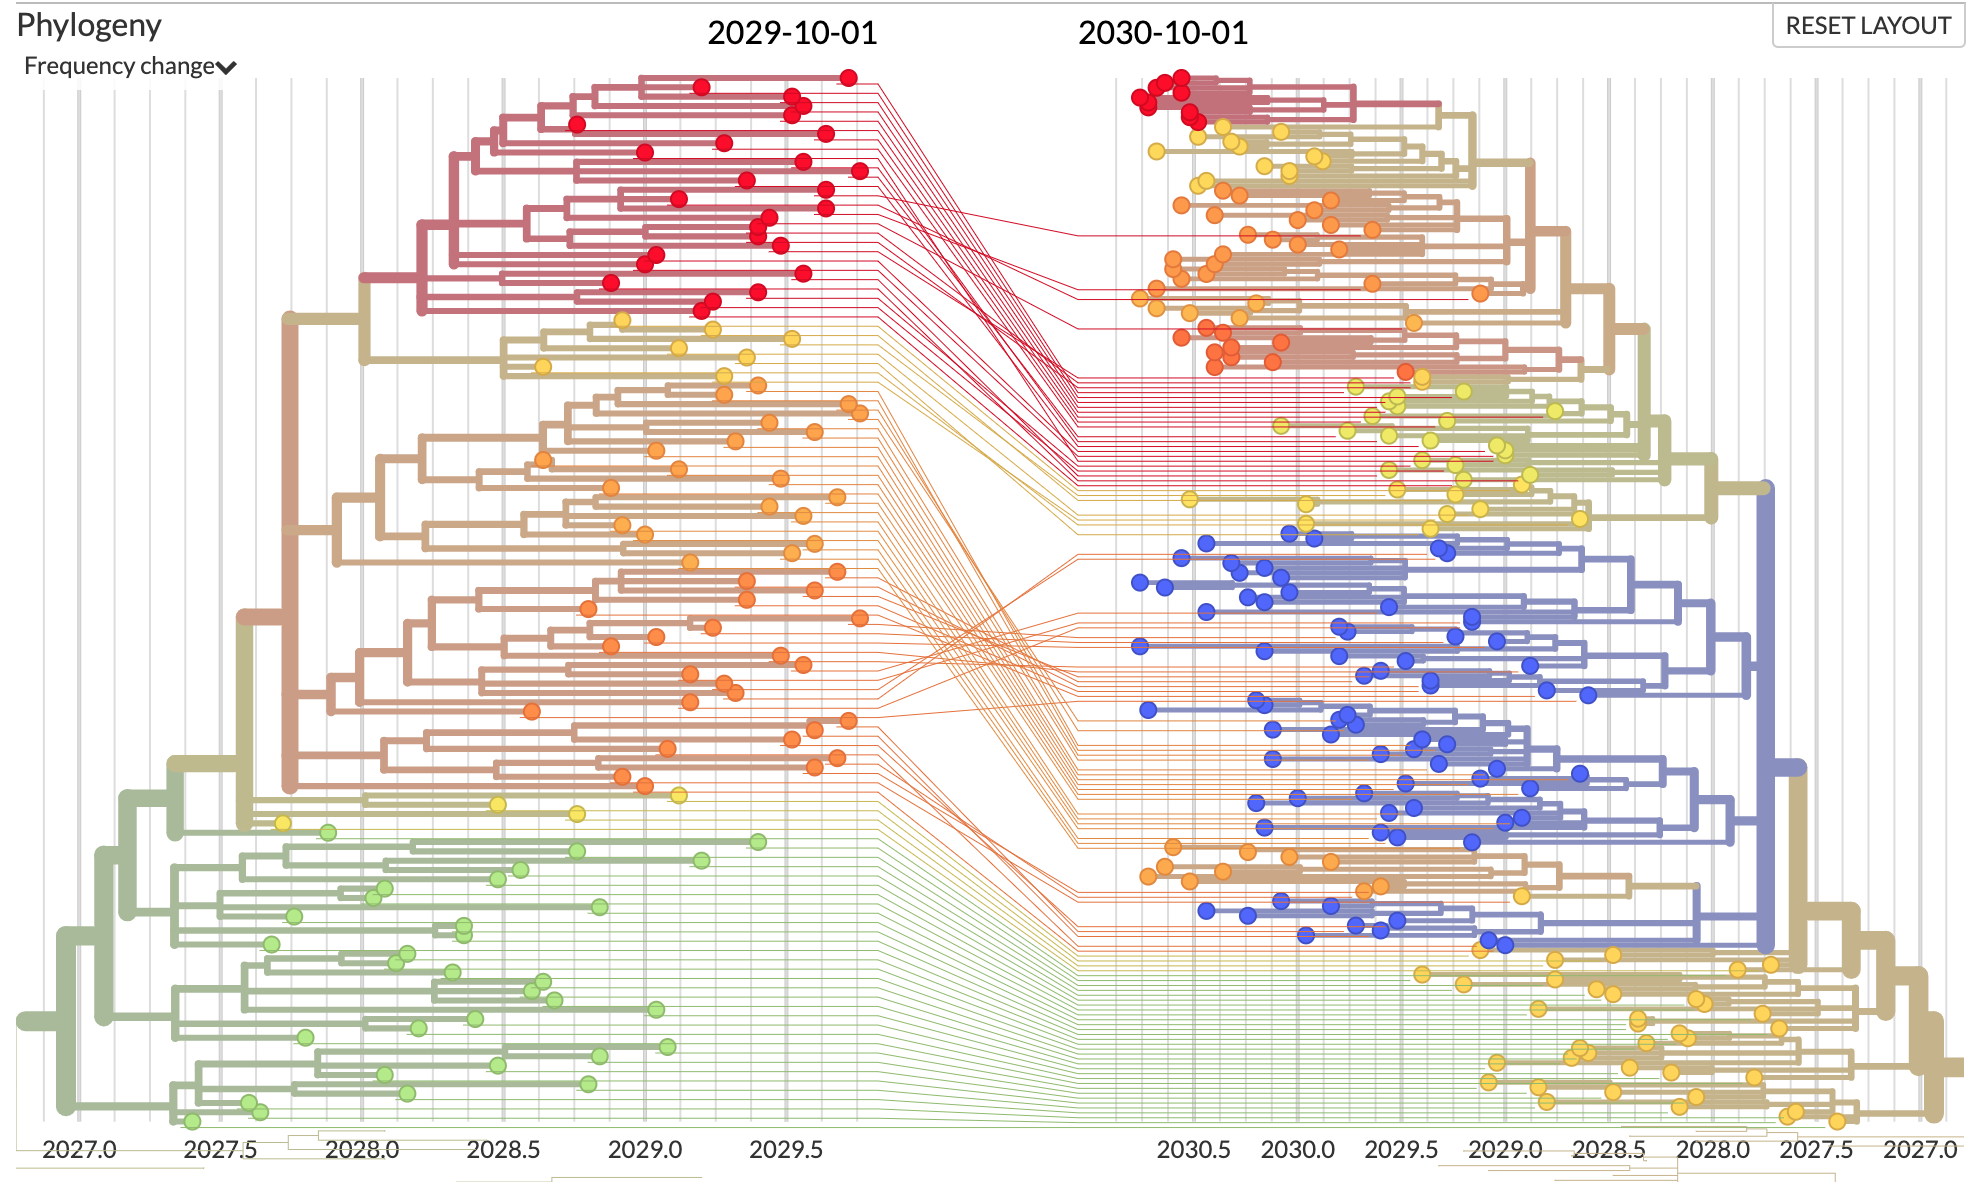
\includegraphics[width=\textwidth]{figures/model.png}
  \caption{Schematic representation of the fitness model.}
  \label{fig:model}
  \end{center}
\end{figure*}

\textit{Brief summary of model implementation here including reference to Fig.~\ref{fig:model}.}

\section*{Results}

\subsection*{Models accurately forecast evolution of simulated populations of {A/H3N2-like viruses}}

The long-term evolution of influenza A/H3N2 hemagglutinin has been previously described as a balance between positive selection for substitutions at epitopes that enable escape from adaptive immunity and purifying selection on domains required to maintain the protein's primary functions of binding and membrane fusion \cite{Bush:1999vj,Neher2013,Luksza:2014hj,Koelle:2015dh}.
To test the ability of our models to accurately detect these evolutionary patterns under controlled conditions, we simulated the long-term evolution of A/H3N2-like viruses under purifying and positive selection for 30 years (Methods).
These selective constraints produced phylogenetic structures and accumulation of epitope and non-epitope mutations that were consistent with phylogenies of natural A/H3N2 HA (Supplemental Figure \ref{sup_fig:simulated_h3n2_ha_phylogeny}).

We hypothesized that fitness metrics associated with viral success such as epitope cross-immunity, LBI, and delta frequency would be assigned positive coefficients, while the non-epitope mutations metric would be assigned a negative coefficient.
We reasoned that both LBI and delta frequency would individually outperform the mechanistic metrics as both of these growth metrics estimate recent clade success regardless of the mechanistic basis for that success.
Correspondingly, we expected that a combined model of epitope cross-immunity and non-epitope mutations would perform as well as or better than the growth metrics.
In addition to these four estimates of viral fitness, we tested models based on both the true fitness of each sample as measured by the simulator and a naive model under which there was no estimated change in population composition over the one year forecasting period.
To control for genetic diversity within and between seasons, we evaluated all model forecasts by the average distance between the estimated and observed future population sequences (Methods).

\begin{figure*}[t]
  \begin{center}
  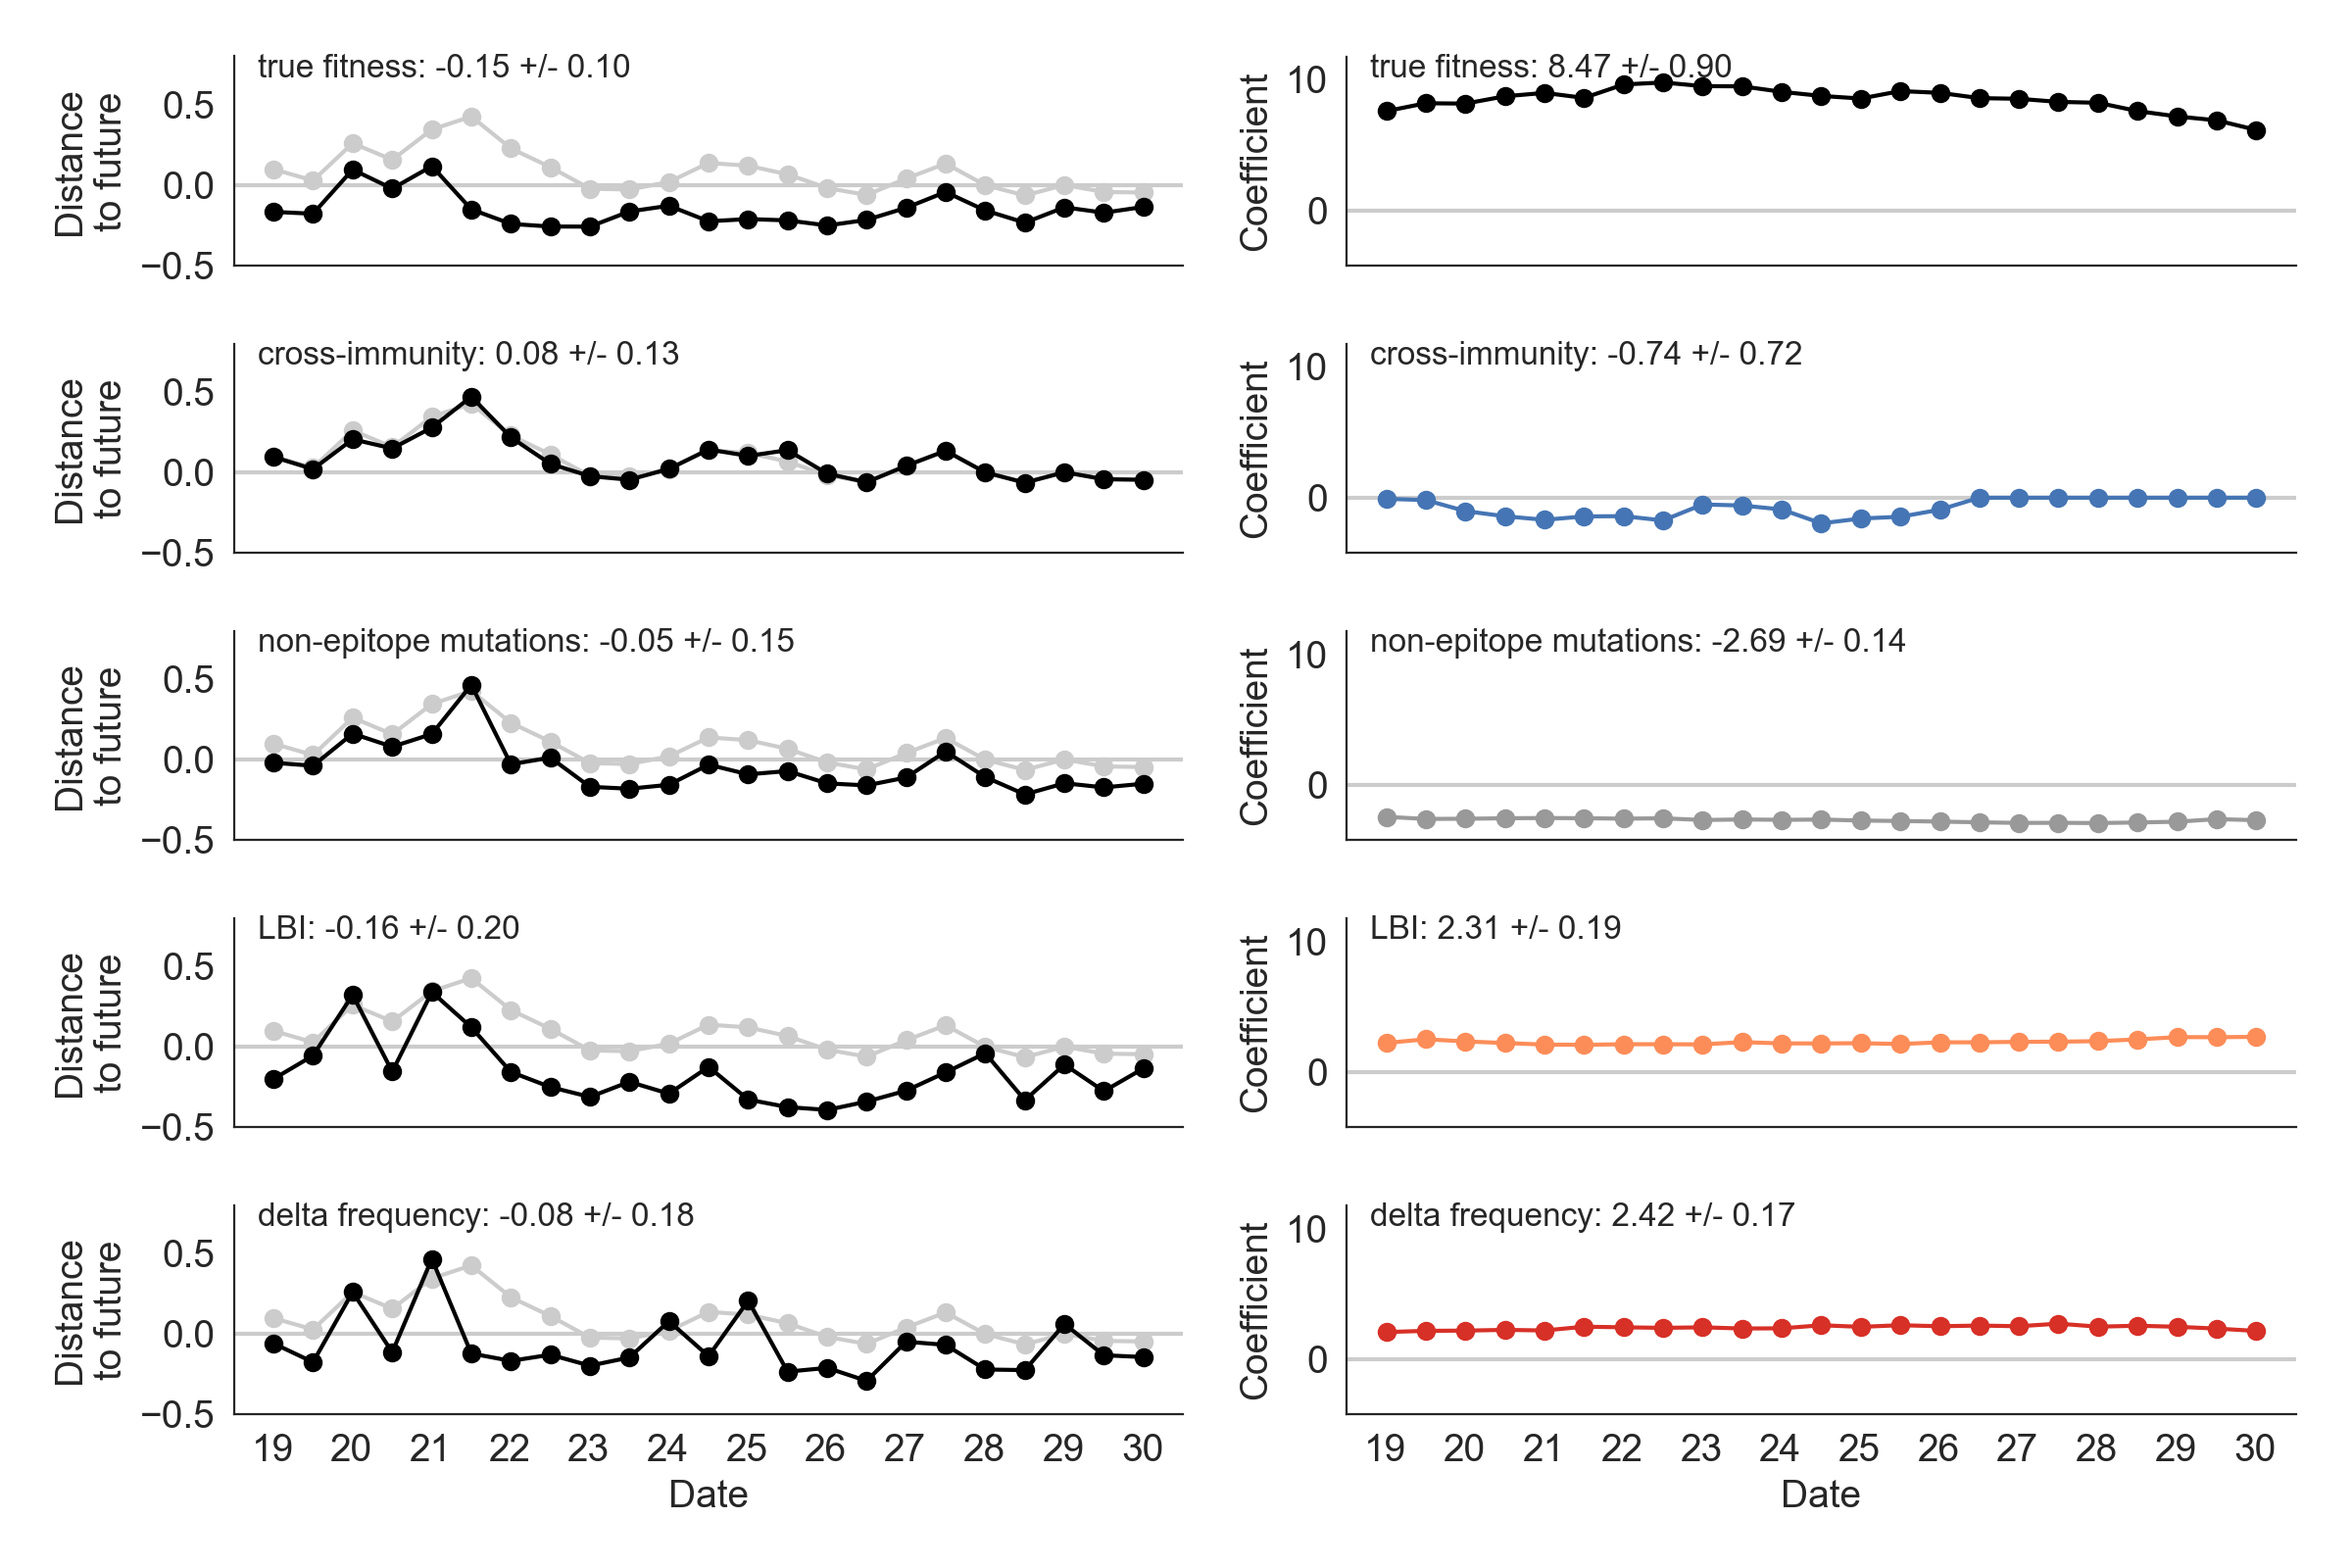
\includegraphics[width=\textwidth]{figures/unadjusted-model-accuracy-and-coefficients-for-simulated-populations.png}
  \caption{Model a) accuracy and b) coefficients for simulated populations of A/H3N2-like viruses.}
  \label{fig:unadjusted_model_accuracy_and_coefficients_for_simulated_populations}
  \end{center}
\end{figure*}

As expected, the true fitness model was the most consistently accurate, estimating distances to the future less than or equal to zero at 21 of 23 (91\%) timepoints (Fig.~\ref{fig:unadjusted_model_accuracy_and_coefficients_for_simulated_populations}).
The naive model was the least accurate, with only seven estimates of zero or less (30\% of timepoints) and an average estimated distance of 0.08 +/- 0.13 (Supplemental Fig.~\ref{sup_fig:distance_of_simulated_populations_between_timepoints}).
Three of the four biologically-informed models performed as expected with the exception of epitope cross-immunity.
LBI and delta frequency both received positive coefficients and outperformed the mechanistic metrics on average.
The non-epitope mutations metric received a consistently negative coefficient and also outperformed the naive model with an average distance less than zero.
Surprisingly, epitope cross-immunity performed no better than the naive model and received a negative average coefficient, despite the anticipated benefit of epitope mutations that could escape exposure-dependent fitness penalties.
Similarly, the combined model of epitope cross-immunity and non-epitope mutations did not perform better than the individual non-epitope mutations model (Supplemental Fig.~\ref{sup_fig:unadjusted_composite_model_accuracy_and_coefficients_for_simulated_populations}).
From these results, we concluded that our models accurately estimate the evolution of simulated populations, but that the fitness of samples under our simulated conditions is dominated by purifying selection rather than by positive selection at epitope sites.

To determine which evolutionary constraints LBI represented, we fit two additional composite models including LBI and non-epitope mutations and LBI with both mutation metrics.
We reasoned that the coefficients learned by these composite models should reflect the relative contribution of each individual metric to the model accuracy.
For example, if LBI measures antigenic advance, we would expect the values of the LBI and cross-immunity coefficients to be mutually exclusive such that increase in LBI coefficient is associated with decrease in the cross-immunity coefficient (Supplemental Fig.~\ref{sup_fig:unadjusted_composite_model_accuracy_and_coefficients_for_simulated_populations}).
Interestingly, we found that the coefficients of the mutation metrics were almost always zero while the LBI coefficients were nearly identical to the coefficients of the individual LBI model.
These results indicate that the predictive contributions of both cross-immunity and non-epitope mutations can be accounted for by LBI alone.

\textit{Repeat simulations with multiple epochs to show model coefficients can reflect these underlying changes to evolutionary constraints.}

\subsection*{Phylogenetic metrics most accurately forecast natural populations of A/H3N2 viruses}

The average distance per year between natural populations was twice that of simulated populations at 0.20 +/- 0.16 (Supplemental Fig.~\ref{sup_fig:distance_of_natural_populations_between_timepoints}).
Consistent with the simulated population results, almost all biologically-informed metrics performed better than the naive model for natural populations with the exception of the cross-immunity metric (Fig.~\ref{fig:unadjusted_model_accuracy_and_coefficients_for_natural_populations}).
The two phylogenetic metrics, LBI and delta frequency, performed consistently better than all other metrics with average distances to the future of -0.06 +/- 0.20 and 0.00 +/- 0.12, respectively.
Importantly, HI phenotypes produced more accurate estimates of the future than the other antigenic metric of cross-immunity.
Variability in the coefficient for the HI phenotypes metric was consistent with relatively sparse HI titer measurements prior to 2011.
In contrast, the sequence-based metric for functional constraint, non-epitope mutations, outperformed the DMS-based phenotypic metric.
The gradual decline of the DMS metric's coefficient around 2009 is consistent with overfitting models to the original background strain of the DMS experiments, A/Perth/16/2009.

\begin{figure*}[t]
  \begin{center}
  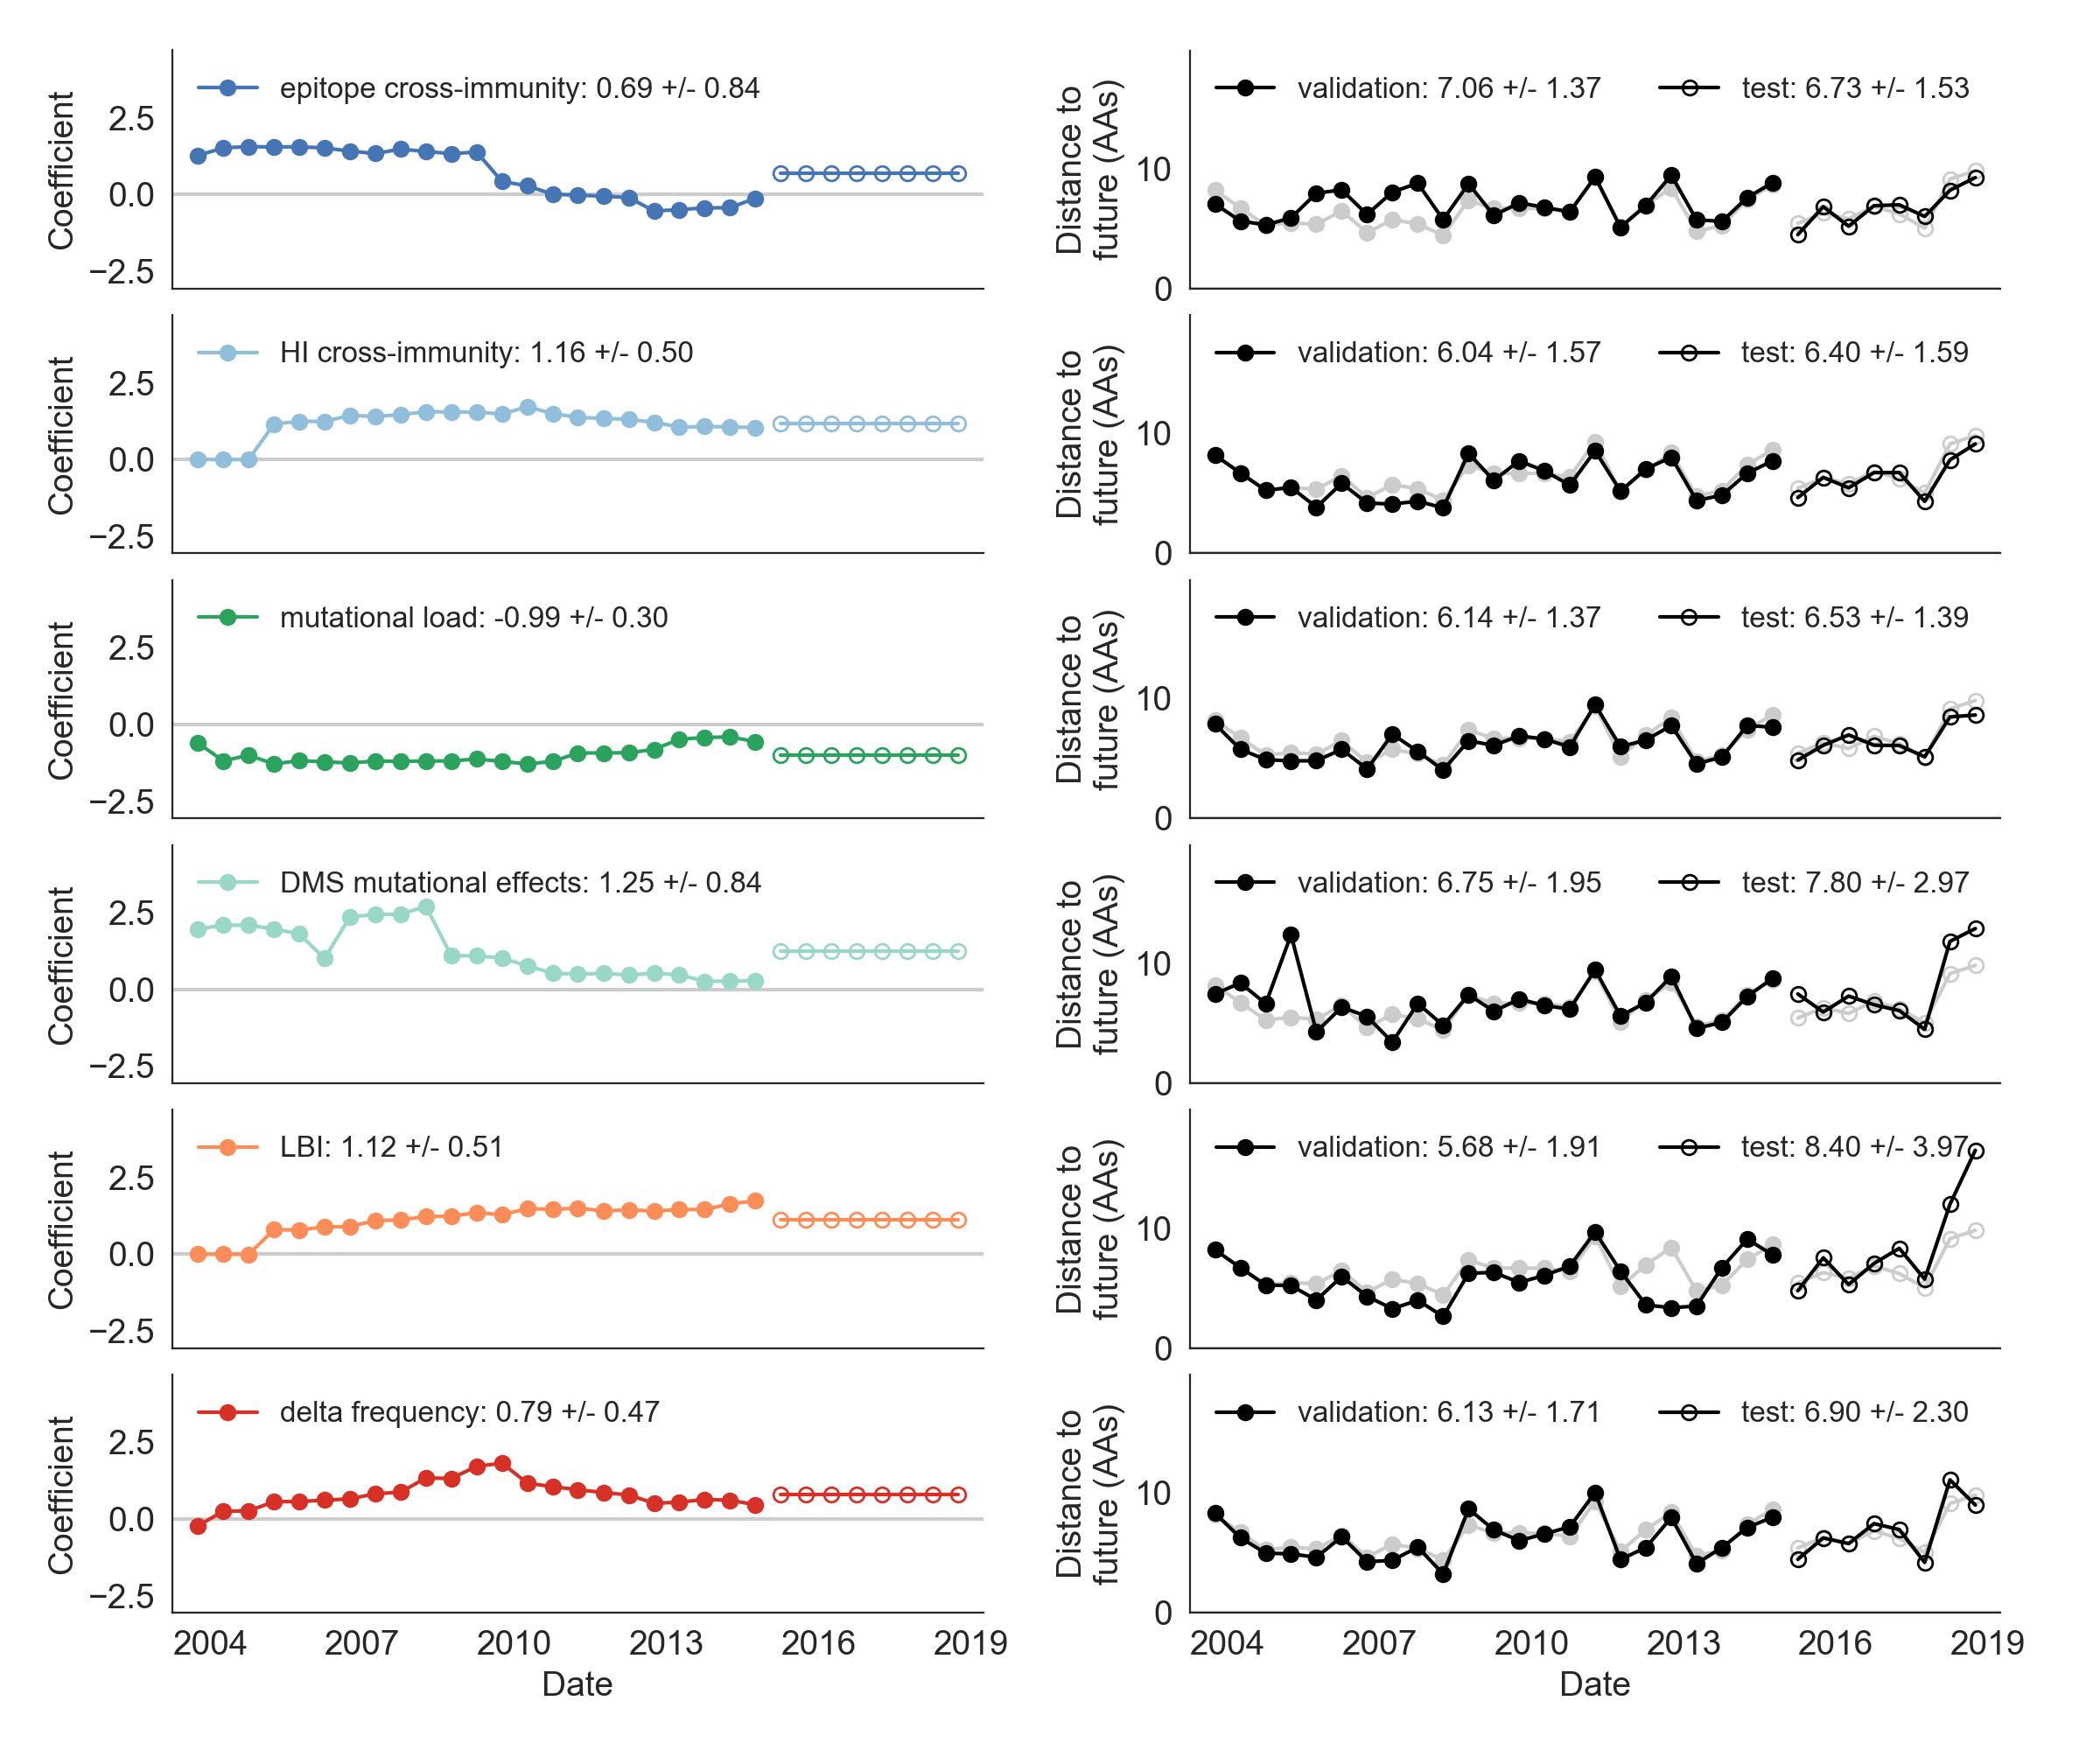
\includegraphics[width=\textwidth]{figures/unadjusted-model-accuracy-and-coefficients-for-natural-populations.png}
  \caption{Model a) accuracy and b) coefficients for natural populations of A/H3N2 viruses.}
  \label{fig:unadjusted_model_accuracy_and_coefficients_for_natural_populations}
  \end{center}
\end{figure*}

The results suggested that combinations of the best individual metrics like LBI, delta frequency, non-epitope mutations, and HI phenotypes could produce even more accurate models.
To this end, we fit models for X combinations of these metrics and evaluated their distance to the future and coefficients relative to the corresponding individual metrics.
We found results (Supplemental Fig.~\ref{sup_fig:unadjusted_composite_model_accuracy_and_coefficients_for_natural_populations}).

\subsection*{Model accuracy and coefficients reflect historical patterns of A/H3N2 evolution}

\subsection*{Composite models outperform models with individual fitness metrics}

\subsection*{Models enable selection of vaccine candidate strains}

\subsection*{Forecasts predict the rise of 3c3.A and A1b clades in February 2020}

\section*{Discussion}

Discussion.

\section*{Methods}

\subsection*{Simulation of influenza A/H3N2-like populations}

We simulated the long-term evolution of A/H3N2-like viruses with SANTA-SIM \cite{Jariani2019} for 40 years where 100 generations was equivalent to 1 year.
We discarded the first 10 years as a burn-in period, selected the next 20 years for model fitting and validation, and held out the last 10 years as out-of-sample data for model testing.
Each simulated population was seeded with the full length HA from A/Beijing/32/1992 (NCBI accession: U26830.1) such that all simulated sequences contained signal peptide, HA1, and HA2 domains.
We defined purifying selection across all three domains, allowing the preferred amino acid at each site to change at a fixed rate over time.
We additionally defined exposure-dependent selection for 49 putative epitope sites in HA1 \cite{Luksza:2014hj} to impose an effect of cross-immunity that would allow mutations at those sites to increase viral fitness despite underlying purifying selection.
We modified the SANTA-SIM source code to enable the inclusion of true fitness values for each sample in the FASTA header of the sampled sequences from each generation.
This modified implementation is available at https://github.com/huddlej/santa-sim/tree/emit-fitness.


\subsection*{Strain selection for natural populations}

For model training and validation, we selected XX HA sequences of length >=1,700 nucleotides that were sampled between October 1994 and October 2015.
To account for known variation in sequence availability by region, we subsampled the selected sequences to a representative set of 10 viruses per month with even sampling across 10 global regions including Africa, Europe, North America, China, South Asia, Japan and Korea, Oceania, South America, Southeast Asia, and West Asia.
We excluded all samples with ambiguous year, month, and day annotations and prioritized samples with more available HI titer measurements.

For model testing, we extended the set of training and validation sequences to include HA sequences that were sampled between October 2015 and April 2019.
We used these test sequences to evaluate the out-of-sample error of fixed model parameters learned during training and validation.

\subsection*{Phylogenetic interference}

For each timepoint in model training, validation, and testing, we selected the subsampled HA sequences with collection dates up to that timepoint.
We aligned sequences with the augur align command \cite{Hadfield2018} and MAFFT v7.407 \cite{Katoh2002}.
We inferred initial phylogenies for HA sequences at each timepoint with IQ-TREE v1.6.10 \cite{Nguyen2014}.
To reconstruct time-resolved phylogenies, we applied TreeTime v0.5.6 \cite{Sagulenko2018} with the augur refine command.

\subsection*{Frequency estimation}

To account for uncertainty in collection date and sampling error, we applied a kernel density estimation (KDE) approach to calculate global sample frequencies.
Specifically, we constructed a Gaussian kernel for each sample with the mean at the reported collection date and a variance of one month, roughly corresponding to the average lag time between sample collection and submission to the GISAID database.
We estimated the frequency of each sample at each timepoint by calculating the cumulative density function of each KDE between the current and previous timepoint and normalizing the resulting values to sum to one.
We implemented this logic in the augur frequencies command.

\subsection*{Model fitting and evaluation}

\subsubsection*{Fitness model}

As in \cite{Luksza:2014hj}, we assumed that influenza A/H3N2 populations can be described by an exponential growth model.
Under this model, we estimated the future frequency of the global population, $\hat{X}$, at some time in the future, $t + \Delta{t}$, based on the current frequency, $x_{i}(t)$, and fitness, $f_{i}(t)$, of each sample $i$ as follows where the resulting future frequencies were normalized to one by $\frac{1}{Z(t)}$.

$$
\hat{X}(t + \Delta{t}) = \frac{1}{Z(t)}\sum_{i}x_{i}(t)\exp(f_{i}(t))
$$

We defined the fitness of each sample at time $t$ as the additive combination of one or more fitness metrics, $f_{i,m}$, scaled by fitness coefficients, $\beta_{m}$.

\subsubsection*{Model target}

For a model based on any given combination of fitness metrics, we found the fitness coefficients that minimized the mean weighted Hamming distance between the estimated and observed future populations at time $u = t + \Delta{t}$ as defined by,

$$
\Delta(X(u), \hat{X}(u)) = \frac{\sum_{i}\sum_{j}x_{i}(t)\exp(f_{i}(t)\Delta{t})x_{j}(u)d_{i,j} - \sum_{j}\sum_{k}x_{j}(u)x_{k}(u)d_{j,k}}{\sum_{i}\sum_{j}x_{i}(t)x_{j}(u)d_{i,j}}.
$$

The first term in the numerator measures the mean distance between estimated and observed future populations, the second term measures the average distance of the future population to itself, and the denominator measures the average distance between the current and future populations.
When a model accurately estimates the average distance of the future population to itself, the metric evaluates to zero.
When the estimated sequence diversity is closer to the center of the future population's observed diversity, the metric evaluates to a negative proportion.
We applied the Nelder-Mead minimization algorithm as implemented in SciPy \cite{SciPy} to learn fitness coefficients that minimize the average of this distance metric over all timepoints in a given training window.

\subsubsection*{Time-series cross-validation}

To obtain unbiased estimates for the out-of-sample errors of our models, we adopted the standard cross-validation strategy of training, validation, and testing.
We divided our available data into an initial training and validation set spanning October 1994 to October 2015 and an additional testing set spanning October 2015 to April 2019.
We partitioned our training and validation data into six month seasons corresponding to winter in the Northern Hemisphere (October--April) and the Southern Hemisphere (April--October) and trained models to estimate frequencies of populations one year into the future from each season in six-year sliding windows.
To calculate validation error for each training window, we applied the resulting model coefficients to estimate the future frequencies for the year after the last timepoint in the training window.
These validation errors informed our tuning of hyperparameters including a L1 regularization of the fitness coefficients, the LBI neighborhood parameter $\tau$, and the length of the training window itself.
Finally, we fixed the coefficients for each model at the mean values across all training windows and applied these fixed models to the test data to estimate the true forecasting accuracy of each model on previously unobserved data.

\subsection*{Fitness metrics}

\subsubsection*{Antigenic drift}

\subsubsection*{Functional constraint}

\subsubsection*{Clade growth}
